%=======================================================================
% Congestion-Aware Joint Charging-Station Placement, Capacity, and
% Swarm-UAV Trajectory Design for Age-Optimal Data Collection
% Target: IEEE Internet of Things Journal (IoT-J)
%=======================================================================
\documentclass[journal]{IEEEtran}

\usepackage{amsmath,amssymb,amsfonts}
\usepackage{algorithmic}
\usepackage{graphicx}
\usepackage{textcomp}
\usepackage{xcolor}
\usepackage{booktabs}
\usepackage{tikz}
\usepackage{pgfplots}
\pgfplotsset{compat=1.18}
\usetikzlibrary{arrows.meta,positioning,fit,backgrounds,calc,shapes.geometric}

\usepackage[colorlinks=true,allcolors=blue]{hyperref}

% --- convenience macros ---
\newtheorem{proposition}{Proposition}
\newtheorem{theorem}{Theorem}
\newtheorem{lemma}{Lemma}
\DeclareMathOperator*{\argmin}{arg\,min}
\newcommand{\Aoi}{\mathrm{AoI}}
\newcommand{\Wq}{W_{\mathrm q}}

\begin{document}

\title{Congestion-Aware Joint Charging-Station Placement, Capacity, and
Swarm-UAV Trajectory Design for Age-Optimal Data Collection}

\author{Do~Phuc~Hao%
\thanks{D.~P.~Hao is with the Center for Artificial Intelligence Research and
Application (CAIRA), Da Nang Architecture University, Da Nang, Vietnam
(e-mail: haodp.ai@gmail.com).}}

\markboth{IEEE Internet of Things Journal, Draft}%
{Hao: Congestion-Aware Joint Placement, Capacity, and Swarm-UAV Trajectory for Age-Optimal Data Collection}

\maketitle

\begin{abstract}
% TODO (fill after results): 200-250 words.
% Motivation: fresh data collection by UAV swarms; energy-limited UAVs must
% recharge at a small number of shared charging stations. Gap: existing works
% treat charging as a single fixed facility or an open queue. Contribution:
% (i) a joint charging-station placement, port-capacity, swarm-trajectory and
% assignment formulation under a DES-validated finite-source (machine-repair)
% charging queue; (ii) two structural results: a congestion threshold making
% AoI non-monotone in swarm size, and a placement inversion (traffic-driven vs
% coverage-driven); (iii) a GPU trajectory optimiser and a block-coordinate
% solver. Results placeholder.
\end{abstract}

\begin{IEEEkeywords}
Age of Information, unmanned aerial vehicles, UAV swarm, data collection,
charging-station placement, finite-source queue, trajectory optimization,
Internet of Things.
\end{IEEEkeywords}

%=======================================================================
\section{Introduction}
\label{sec:intro}
% TODO: motivation, gap, contributions bullet list, paper organisation.
% Contributions:
% C1) First joint placement + port-capacity + swarm-trajectory + assignment
%     formulation for peak-AoI fresh data collection with a CONTENDED,
%     multi-server charging resource.
% C2) A DES-validated finite-source (machine-repair) queue model; we show the
%     open M/M/c over-predicts wait ~6x and distorts decisions.
% C3) Proposition 1 (congestion threshold: AoI non-monotone in swarm size) and
%     Proposition 2 (placement inversion: coverage-optimal is suboptimal).
% C4) A GPU CETSP trajectory optimiser and a block-coordinate joint solver;
%     evaluation vs single-UAV / single-station / coverage baselines.

%=======================================================================
\section{Related Work}
\label{sec:related}
\subsection{AoI-oriented UAV data collection}
The Age of Information (AoI) was introduced in \cite{kaul2012aoi} as a
destination-centric measure of data freshness, capturing the time elapsed
since the generation of the most recently received update. AoI has since
become a standard objective for UAV-assisted data collection, where a UAV
visits distributed sources and the design goal is to keep the collected
information fresh. In the swarm setting, \cite{eldeeb2023swarm} minimizes AoI
across multiple cooperating UAVs using multi-agent reinforcement learning,
demonstrating that coordinated trajectories can reduce peak AoI relative to
uncoordinated flight. That formulation, however, assumes flight endurance is
unconstrained: it carries no energy state and no recharging model, so the
depletion and replenishment dynamics that dominate long missions are absent.
Closest to our objective is \cite{base2024}, which jointly optimizes charging
station placement, UAV trajectory, and peak AoI, and which we adopt as our
point of departure. That work is nonetheless single-UAV: with one vehicle
there is no inter-UAV contention for a charger, no need for multi-port
capacity, and no swarm assignment, precisely the coupling that our design
targets.

\subsection{Energy-limited UAVs and charging}
A second line of work makes energy replenishment explicit. In \cite{wei2024},
multiple UAVs share a limited charging facility and the resulting charge
waiting time is folded into the AoI objective, then optimized by deep
reinforcement learning. The facility there is single and fixed in location,
which effectively reduces contention to a single-server queue and leaves
station placement out of scope. Laser-based (LBD) charging is studied in
\cite{sun2025laser}, where charging sites are at fixed locations and are
treated without queue contention, so neither where to place stations nor how
many vehicles may wait is optimized. A different tactic uses mobile chargers:
\cite{oubbati2024ugv} and \cite{zhao2025aoi} employ ground vehicles that
follow the UAVs to deliver energy on the move. Because the charger comes to
the UAV, this removes the fixed-station contention that is central to our
setting and does not address the placement of fixed, multi-port stations.
Finally, \cite{ev2022sharing} does model UAV charging stations as a contended
queue and provides a waiting-time analysis, but it optimizes neither AoI nor
trajectory nor station placement, so the queueing model is not coupled to any
freshness or mobility decision.

\subsection{Positioning and gap}
Read together, these works each supply a subset of the ingredients our problem
requires but never their combination. Swarm operation with AoI appears in
\cite{eldeeb2023swarm} yet without charging; placement with AoI appears in
\cite{base2024} yet only for a single UAV; charge waiting is captured in
\cite{wei2024} yet at a single fixed server without placement; and a contended
charging queue is analyzed in \cite{ev2022sharing} yet without AoI,
trajectory, or placement. No prior formulation simultaneously carries all four
of station placement, swarm operation, multi-server charging contention, and a
peak-AoI objective. Our work closes this gap by jointly optimizing station
placement, port capacity, swarm trajectory, and source-to-UAV assignment under
a charging model that is a contended, multi-server, and finite-source (closed)
queue, validated against discrete-event simulation. The finite-source aspect
is not a cosmetic refinement: because the number of UAVs competing for a
station is small and closed, modeling the queue as an open M/M/c system
over-predicts waiting time and thereby distorts both placement and capacity
decisions, an effect we quantify and correct with the finite-source model
detailed in Section~\ref{sec:model}. This coupled formulation also yields two
structural findings that a decoupled treatment cannot expose: a congestion
threshold, beyond which peak AoI is non-monotone in swarm size, and a
placement inversion, whereby coverage-optimal station placement becomes
AoI-suboptimal once contention is accounted for.
   % <-- sub-agent writes this

%=======================================================================
\section{System Model and Problem Formulation}
\label{sec:model}
% Placeholder — sub-agent fills this.
Formulation goes here.
   % <-- sub-agent writes this

\begin{figure}[t]
  \centering
  \resizebox{\columnwidth}{!}{% System model: swarm-UAV fresh data collection with shared multi-port
% charging stations forming a finite-source (closed) queue.
% Included via \resizebox{\columnwidth}{!}{% System model: swarm-UAV fresh data collection with shared multi-port
% charging stations forming a finite-source (closed) queue.
% Included via \resizebox{\columnwidth}{!}{% System model: swarm-UAV fresh data collection with shared multi-port
% charging stations forming a finite-source (closed) queue.
% Included via \resizebox{\columnwidth}{!}{\input{figs/fig_system_model}}
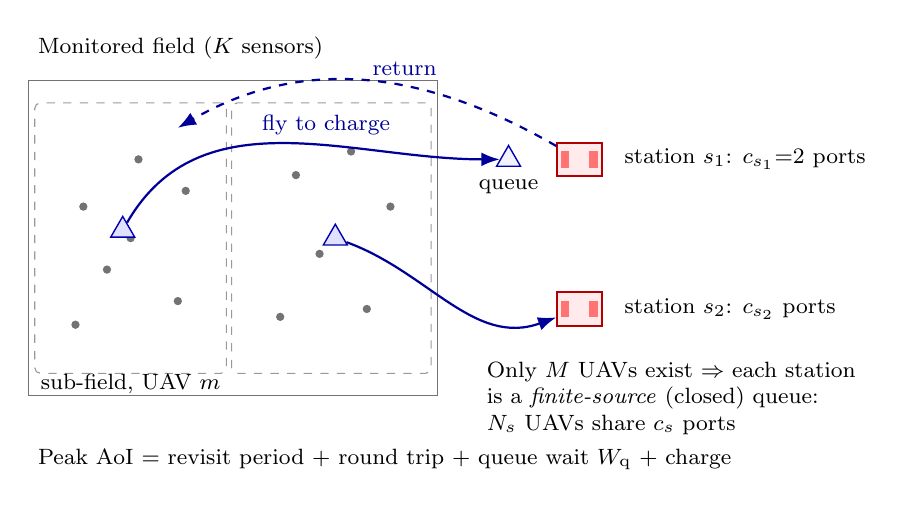
\begin{tikzpicture}[
    >=Latex,
    sensor/.style={circle,fill=black!55,minimum size=3pt,inner sep=0pt},
    uav/.style={regular polygon,regular polygon sides=3,draw=blue!70!black,
                fill=blue!12,minimum size=10pt,inner sep=0pt,line width=0.5pt},
    station/.style={rectangle,draw=red!70!black,fill=red!8,minimum width=16pt,
                    minimum height=12pt,line width=0.7pt},
    port/.style={rectangle,fill=red!55,minimum width=3pt,minimum height=6pt,inner sep=0pt},
    subfield/.style={draw=black!40,dashed,rounded corners=2pt},
    lbl/.style={font=\footnotesize},
    flow/.style={->,thick,blue!60!black},
]

% ---- monitored field with two sub-fields ----
\node[lbl,anchor=south west] at (0,4.15) {Monitored field ($K$ sensors)};
\draw[black!55] (0,0) rectangle (5.2,4);

% sub-field A (left) with sensors + UAV
\node[subfield,fit={(0.2,0.4)(2.4,3.6)}] (sfA) {};
\foreach \p in {(0.6,0.9),(1.0,1.6),(0.7,2.4),(1.4,3.0),(1.9,1.2),(2.0,2.6),(1.3,2.0)}
  \node[sensor] at \p {};
\node[uav] (uA) at (1.2,2.1) {};
\node[lbl] at (1.3,0.15) {sub-field, UAV $m$};

% sub-field B (right)
\node[subfield,fit={(2.7,0.4)(5.0,3.6)}] (sfB) {};
\foreach \p in {(3.2,1.0),(3.7,1.8),(4.3,1.1),(4.6,2.4),(3.4,2.8),(4.1,3.1),(3.9,2.0)}
  \node[sensor] at \p {};
\node[uav] (uB) at (3.9,2.0) {};

% ---- two charging stations with ports + a short queue ----
\node[station] (s1) at (7.0,3.0) {};
\node[port] at ($(s1)+(-0.18,0)$) {};
\node[port] at ($(s1)+(0.18,0)$) {};
\node[lbl,anchor=west] at ($(s1)+(0.45,0)$) {station $s_1$: $c_{s_1}{=}2$ ports};
\node[uav,fill=blue!5] (q1) at ($(s1)+(-0.9,0)$) {};   % waiting UAV
\node[lbl] at ($(s1)+(-0.9,-0.35)$) {queue};

\node[station] (s2) at (7.0,1.1) {};
\node[port] at ($(s2)+(-0.18,0)$) {};
\node[port] at ($(s2)+(0.18,0)$) {};
\node[lbl,anchor=west] at ($(s2)+(0.45,0)$) {station $s_2$: $c_{s_2}$ ports};

% ---- cycle arrows: patrol -> fly to station -> queue+charge -> return ----
\draw[flow] (uA) to[out=60,in=180] node[lbl,above,pos=0.6]{fly to charge} (q1);
\draw[flow] (uB) to[out=-20,in=200] (s2);
\draw[flow,dashed] (s1) to[out=150,in=30] node[lbl,above,pos=0.4]{return} (1.9,3.4);

% ---- annotations ----
\node[lbl,align=left,anchor=north west] at (5.7,0.55)
  {Only $M$ UAVs exist $\Rightarrow$ each station\\
   is a \emph{finite-source} (closed) queue:\\
   $N_s$ UAVs share $c_s$ ports};
\node[lbl,align=left,anchor=north west] at (0.0,-0.55)
  {Peak $\Aoi$ $=$ revisit period $+$ round trip $+$ queue wait $\Wq$ $+$ charge};

\end{tikzpicture}
}
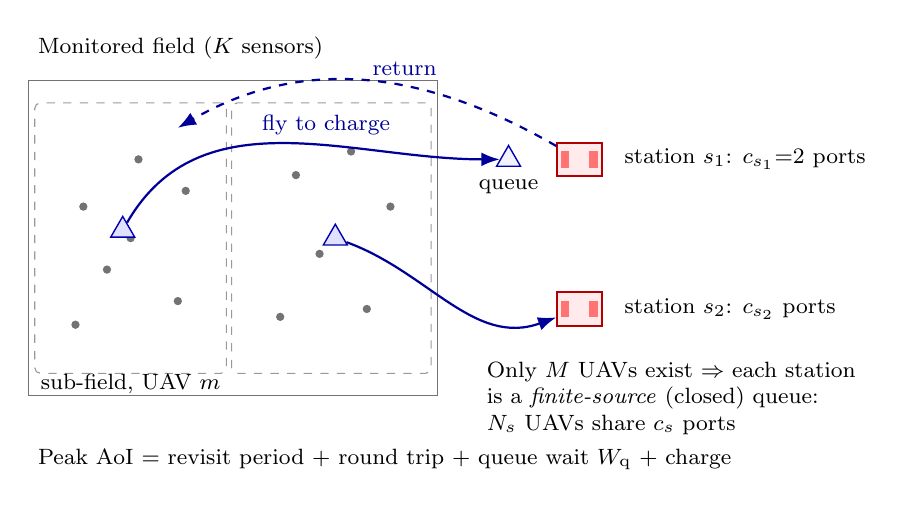
\begin{tikzpicture}[
    >=Latex,
    sensor/.style={circle,fill=black!55,minimum size=3pt,inner sep=0pt},
    uav/.style={regular polygon,regular polygon sides=3,draw=blue!70!black,
                fill=blue!12,minimum size=10pt,inner sep=0pt,line width=0.5pt},
    station/.style={rectangle,draw=red!70!black,fill=red!8,minimum width=16pt,
                    minimum height=12pt,line width=0.7pt},
    port/.style={rectangle,fill=red!55,minimum width=3pt,minimum height=6pt,inner sep=0pt},
    subfield/.style={draw=black!40,dashed,rounded corners=2pt},
    lbl/.style={font=\footnotesize},
    flow/.style={->,thick,blue!60!black},
]

% ---- monitored field with two sub-fields ----
\node[lbl,anchor=south west] at (0,4.15) {Monitored field ($K$ sensors)};
\draw[black!55] (0,0) rectangle (5.2,4);

% sub-field A (left) with sensors + UAV
\node[subfield,fit={(0.2,0.4)(2.4,3.6)}] (sfA) {};
\foreach \p in {(0.6,0.9),(1.0,1.6),(0.7,2.4),(1.4,3.0),(1.9,1.2),(2.0,2.6),(1.3,2.0)}
  \node[sensor] at \p {};
\node[uav] (uA) at (1.2,2.1) {};
\node[lbl] at (1.3,0.15) {sub-field, UAV $m$};

% sub-field B (right)
\node[subfield,fit={(2.7,0.4)(5.0,3.6)}] (sfB) {};
\foreach \p in {(3.2,1.0),(3.7,1.8),(4.3,1.1),(4.6,2.4),(3.4,2.8),(4.1,3.1),(3.9,2.0)}
  \node[sensor] at \p {};
\node[uav] (uB) at (3.9,2.0) {};

% ---- two charging stations with ports + a short queue ----
\node[station] (s1) at (7.0,3.0) {};
\node[port] at ($(s1)+(-0.18,0)$) {};
\node[port] at ($(s1)+(0.18,0)$) {};
\node[lbl,anchor=west] at ($(s1)+(0.45,0)$) {station $s_1$: $c_{s_1}{=}2$ ports};
\node[uav,fill=blue!5] (q1) at ($(s1)+(-0.9,0)$) {};   % waiting UAV
\node[lbl] at ($(s1)+(-0.9,-0.35)$) {queue};

\node[station] (s2) at (7.0,1.1) {};
\node[port] at ($(s2)+(-0.18,0)$) {};
\node[port] at ($(s2)+(0.18,0)$) {};
\node[lbl,anchor=west] at ($(s2)+(0.45,0)$) {station $s_2$: $c_{s_2}$ ports};

% ---- cycle arrows: patrol -> fly to station -> queue+charge -> return ----
\draw[flow] (uA) to[out=60,in=180] node[lbl,above,pos=0.6]{fly to charge} (q1);
\draw[flow] (uB) to[out=-20,in=200] (s2);
\draw[flow,dashed] (s1) to[out=150,in=30] node[lbl,above,pos=0.4]{return} (1.9,3.4);

% ---- annotations ----
\node[lbl,align=left,anchor=north west] at (5.7,0.55)
  {Only $M$ UAVs exist $\Rightarrow$ each station\\
   is a \emph{finite-source} (closed) queue:\\
   $N_s$ UAVs share $c_s$ ports};
\node[lbl,align=left,anchor=north west] at (0.0,-0.55)
  {Peak $\Aoi$ $=$ revisit period $+$ round trip $+$ queue wait $\Wq$ $+$ charge};

\end{tikzpicture}
}
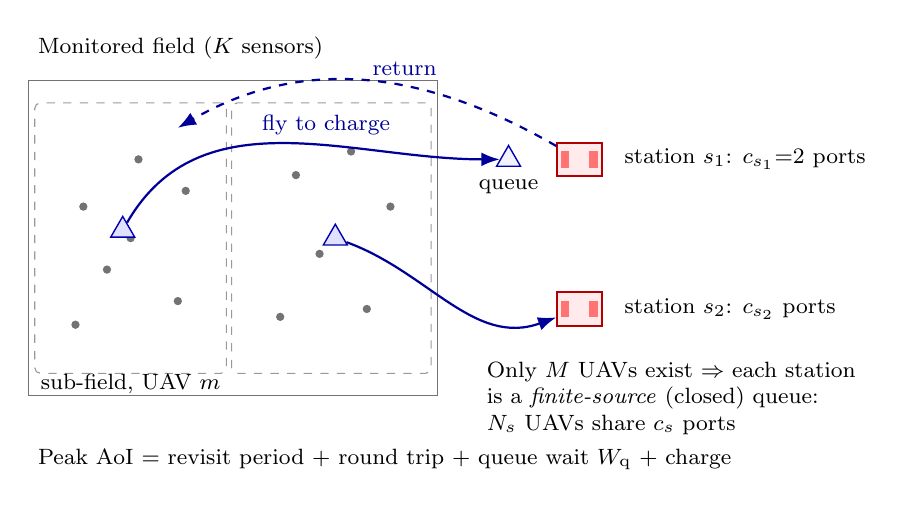
\begin{tikzpicture}[
    >=Latex,
    sensor/.style={circle,fill=black!55,minimum size=3pt,inner sep=0pt},
    uav/.style={regular polygon,regular polygon sides=3,draw=blue!70!black,
                fill=blue!12,minimum size=10pt,inner sep=0pt,line width=0.5pt},
    station/.style={rectangle,draw=red!70!black,fill=red!8,minimum width=16pt,
                    minimum height=12pt,line width=0.7pt},
    port/.style={rectangle,fill=red!55,minimum width=3pt,minimum height=6pt,inner sep=0pt},
    subfield/.style={draw=black!40,dashed,rounded corners=2pt},
    lbl/.style={font=\footnotesize},
    flow/.style={->,thick,blue!60!black},
]

% ---- monitored field with two sub-fields ----
\node[lbl,anchor=south west] at (0,4.15) {Monitored field ($K$ sensors)};
\draw[black!55] (0,0) rectangle (5.2,4);

% sub-field A (left) with sensors + UAV
\node[subfield,fit={(0.2,0.4)(2.4,3.6)}] (sfA) {};
\foreach \p in {(0.6,0.9),(1.0,1.6),(0.7,2.4),(1.4,3.0),(1.9,1.2),(2.0,2.6),(1.3,2.0)}
  \node[sensor] at \p {};
\node[uav] (uA) at (1.2,2.1) {};
\node[lbl] at (1.3,0.15) {sub-field, UAV $m$};

% sub-field B (right)
\node[subfield,fit={(2.7,0.4)(5.0,3.6)}] (sfB) {};
\foreach \p in {(3.2,1.0),(3.7,1.8),(4.3,1.1),(4.6,2.4),(3.4,2.8),(4.1,3.1),(3.9,2.0)}
  \node[sensor] at \p {};
\node[uav] (uB) at (3.9,2.0) {};

% ---- two charging stations with ports + a short queue ----
\node[station] (s1) at (7.0,3.0) {};
\node[port] at ($(s1)+(-0.18,0)$) {};
\node[port] at ($(s1)+(0.18,0)$) {};
\node[lbl,anchor=west] at ($(s1)+(0.45,0)$) {station $s_1$: $c_{s_1}{=}2$ ports};
\node[uav,fill=blue!5] (q1) at ($(s1)+(-0.9,0)$) {};   % waiting UAV
\node[lbl] at ($(s1)+(-0.9,-0.35)$) {queue};

\node[station] (s2) at (7.0,1.1) {};
\node[port] at ($(s2)+(-0.18,0)$) {};
\node[port] at ($(s2)+(0.18,0)$) {};
\node[lbl,anchor=west] at ($(s2)+(0.45,0)$) {station $s_2$: $c_{s_2}$ ports};

% ---- cycle arrows: patrol -> fly to station -> queue+charge -> return ----
\draw[flow] (uA) to[out=60,in=180] node[lbl,above,pos=0.6]{fly to charge} (q1);
\draw[flow] (uB) to[out=-20,in=200] (s2);
\draw[flow,dashed] (s1) to[out=150,in=30] node[lbl,above,pos=0.4]{return} (1.9,3.4);

% ---- annotations ----
\node[lbl,align=left,anchor=north west] at (5.7,0.55)
  {Only $M$ UAVs exist $\Rightarrow$ each station\\
   is a \emph{finite-source} (closed) queue:\\
   $N_s$ UAVs share $c_s$ ports};
\node[lbl,align=left,anchor=north west] at (0.0,-0.55)
  {Peak $\Aoi$ $=$ revisit period $+$ round trip $+$ queue wait $\Wq$ $+$ charge};

\end{tikzpicture}
}
  \caption{System model: a UAV swarm patrols sub-fields to keep sensor data
  fresh, and recharges at a small number of shared, multi-port charging
  stations. Because only $M$ UAVs exist, the charging stations form a
  \emph{finite-source} (closed) queue.}
  \label{fig:system}
\end{figure}

%=======================================================================
\section{Structural Analysis}
\label{sec:analysis}
% TODO (sub-agent / later): Proposition 1 (congestion threshold, U-shape,
% provisioning law) and Proposition 2 (placement inversion) with proofs.

%=======================================================================
\section{Joint Solver}
\label{sec:solver}
% TODO: block-coordinate solver; CETSP trajectory (GPU); finite-source queue;
% water-filling port allocation; load-balanced assignment; placement search.

\begin{figure}[t]
  \centering
  \resizebox{\columnwidth}{!}{% Block-coordinate joint solver flow.
% Included via \resizebox{\columnwidth}{!}{% Block-coordinate joint solver flow.
% Included via \resizebox{\columnwidth}{!}{% Block-coordinate joint solver flow.
% Included via \resizebox{\columnwidth}{!}{\input{figs/fig_solver_flow}}
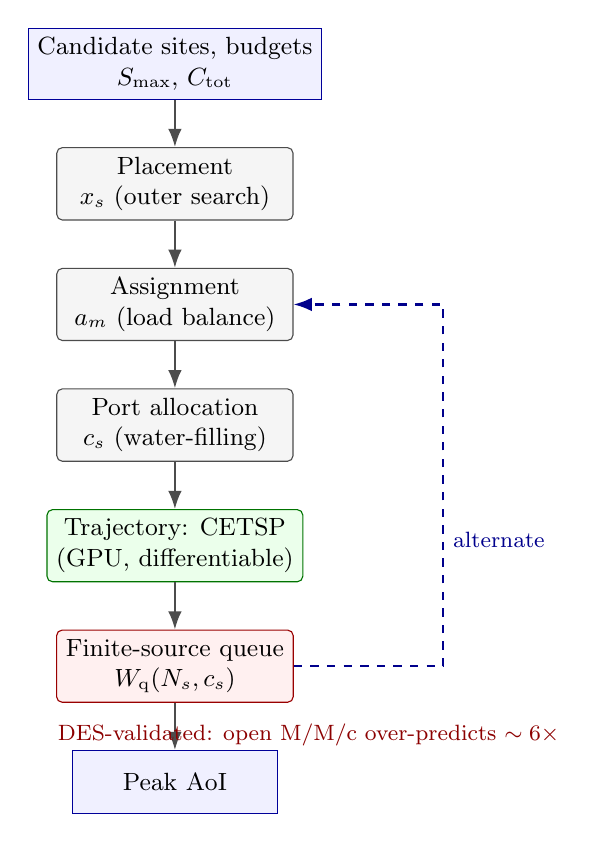
\begin{tikzpicture}[
    >=Latex,
    block/.style={rectangle,rounded corners=2pt,draw=black!70,fill=black!4,
                  minimum width=30mm,minimum height=9mm,align=center,font=\small},
    gpu/.style={rectangle,rounded corners=2pt,draw=green!45!black,fill=green!8,
                minimum width=30mm,minimum height=9mm,align=center,font=\small},
    queue/.style={rectangle,rounded corners=2pt,draw=red!60!black,fill=red!6,
                  minimum width=30mm,minimum height=9mm,align=center,font=\small},
    io/.style={rectangle,draw=blue!60!black,fill=blue!6,minimum width=26mm,
               minimum height=8mm,align=center,font=\small},
    fl/.style={->,thick,black!70},
    lbl/.style={font=\footnotesize},
]

\node[io] (in) {Candidate sites, budgets\\$S_{\max},\,C_{\mathrm{tot}}$};
\node[block,below=6mm of in] (place) {Placement\\$x_s$ (outer search)};
\node[block,below=6mm of place] (assign) {Assignment\\$a_m$ (load balance)};
\node[block,below=6mm of assign] (ports) {Port allocation\\$c_s$ (water-filling)};
\node[gpu,below=6mm of ports] (traj) {Trajectory: CETSP\\(GPU, differentiable)};
\node[queue,below=6mm of traj] (q) {Finite-source queue\\$\Wq(N_s,c_s)$};
\node[io,below=6mm of q] (out) {Peak $\Aoi$};

\draw[fl] (in) -- (place);
\draw[fl] (place) -- (assign);
\draw[fl] (assign) -- (ports);
\draw[fl] (ports) -- (traj);
\draw[fl] (traj) -- (q);
\draw[fl] (q) -- (out);

% block-coordinate loop (right side, back up)
\draw[fl,dashed,blue!55!black]
  (q.east) -- ++(1.9,0) coordinate (turn)
  |- (assign.east);
\node[lbl,blue!55!black,right] at ($(turn)+(0,1.6)$) {alternate};

% DES-validation annotation on the queue block
\node[lbl,align=left,anchor=north west,red!55!black] at ($(q.south west)+(-0.1,-0.15)$)
  {DES-validated: open M/M/c over-predicts $\sim6\times$};

\end{tikzpicture}
}
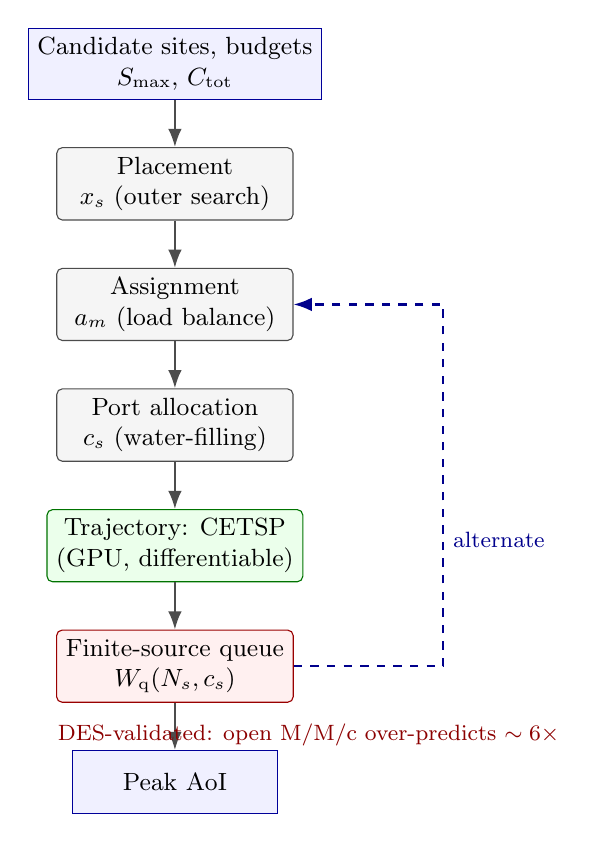
\begin{tikzpicture}[
    >=Latex,
    block/.style={rectangle,rounded corners=2pt,draw=black!70,fill=black!4,
                  minimum width=30mm,minimum height=9mm,align=center,font=\small},
    gpu/.style={rectangle,rounded corners=2pt,draw=green!45!black,fill=green!8,
                minimum width=30mm,minimum height=9mm,align=center,font=\small},
    queue/.style={rectangle,rounded corners=2pt,draw=red!60!black,fill=red!6,
                  minimum width=30mm,minimum height=9mm,align=center,font=\small},
    io/.style={rectangle,draw=blue!60!black,fill=blue!6,minimum width=26mm,
               minimum height=8mm,align=center,font=\small},
    fl/.style={->,thick,black!70},
    lbl/.style={font=\footnotesize},
]

\node[io] (in) {Candidate sites, budgets\\$S_{\max},\,C_{\mathrm{tot}}$};
\node[block,below=6mm of in] (place) {Placement\\$x_s$ (outer search)};
\node[block,below=6mm of place] (assign) {Assignment\\$a_m$ (load balance)};
\node[block,below=6mm of assign] (ports) {Port allocation\\$c_s$ (water-filling)};
\node[gpu,below=6mm of ports] (traj) {Trajectory: CETSP\\(GPU, differentiable)};
\node[queue,below=6mm of traj] (q) {Finite-source queue\\$\Wq(N_s,c_s)$};
\node[io,below=6mm of q] (out) {Peak $\Aoi$};

\draw[fl] (in) -- (place);
\draw[fl] (place) -- (assign);
\draw[fl] (assign) -- (ports);
\draw[fl] (ports) -- (traj);
\draw[fl] (traj) -- (q);
\draw[fl] (q) -- (out);

% block-coordinate loop (right side, back up)
\draw[fl,dashed,blue!55!black]
  (q.east) -- ++(1.9,0) coordinate (turn)
  |- (assign.east);
\node[lbl,blue!55!black,right] at ($(turn)+(0,1.6)$) {alternate};

% DES-validation annotation on the queue block
\node[lbl,align=left,anchor=north west,red!55!black] at ($(q.south west)+(-0.1,-0.15)$)
  {DES-validated: open M/M/c over-predicts $\sim6\times$};

\end{tikzpicture}
}
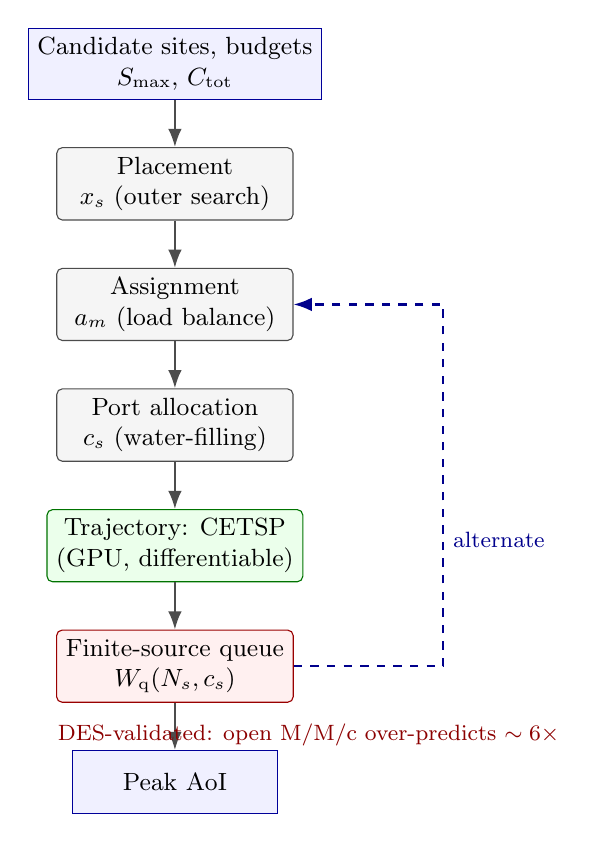
\begin{tikzpicture}[
    >=Latex,
    block/.style={rectangle,rounded corners=2pt,draw=black!70,fill=black!4,
                  minimum width=30mm,minimum height=9mm,align=center,font=\small},
    gpu/.style={rectangle,rounded corners=2pt,draw=green!45!black,fill=green!8,
                minimum width=30mm,minimum height=9mm,align=center,font=\small},
    queue/.style={rectangle,rounded corners=2pt,draw=red!60!black,fill=red!6,
                  minimum width=30mm,minimum height=9mm,align=center,font=\small},
    io/.style={rectangle,draw=blue!60!black,fill=blue!6,minimum width=26mm,
               minimum height=8mm,align=center,font=\small},
    fl/.style={->,thick,black!70},
    lbl/.style={font=\footnotesize},
]

\node[io] (in) {Candidate sites, budgets\\$S_{\max},\,C_{\mathrm{tot}}$};
\node[block,below=6mm of in] (place) {Placement\\$x_s$ (outer search)};
\node[block,below=6mm of place] (assign) {Assignment\\$a_m$ (load balance)};
\node[block,below=6mm of assign] (ports) {Port allocation\\$c_s$ (water-filling)};
\node[gpu,below=6mm of ports] (traj) {Trajectory: CETSP\\(GPU, differentiable)};
\node[queue,below=6mm of traj] (q) {Finite-source queue\\$\Wq(N_s,c_s)$};
\node[io,below=6mm of q] (out) {Peak $\Aoi$};

\draw[fl] (in) -- (place);
\draw[fl] (place) -- (assign);
\draw[fl] (assign) -- (ports);
\draw[fl] (ports) -- (traj);
\draw[fl] (traj) -- (q);
\draw[fl] (q) -- (out);

% block-coordinate loop (right side, back up)
\draw[fl,dashed,blue!55!black]
  (q.east) -- ++(1.9,0) coordinate (turn)
  |- (assign.east);
\node[lbl,blue!55!black,right] at ($(turn)+(0,1.6)$) {alternate};

% DES-validation annotation on the queue block
\node[lbl,align=left,anchor=north west,red!55!black] at ($(q.south west)+(-0.1,-0.15)$)
  {DES-validated: open M/M/c over-predicts $\sim6\times$};

\end{tikzpicture}
}
  \caption{Block-coordinate solver. The trajectory block (GPU CETSP) and the
  finite-source queue are alternated with port allocation, assignment, and an
  outer placement search.}
  \label{fig:solver}
\end{figure}

%=======================================================================
\section{Experiments}
\label{sec:exp}
% TODO (fill from server results): setup, queue-model validation vs DES,
% Prop.1 U-shape + provisioning, Prop.2 placement inversion, joint comparison
% + ablation + Wilcoxon.

% --- result figure placeholders (uncomment when PNGs/CSVs are in) ---
% \begin{figure}[t]\centering
%   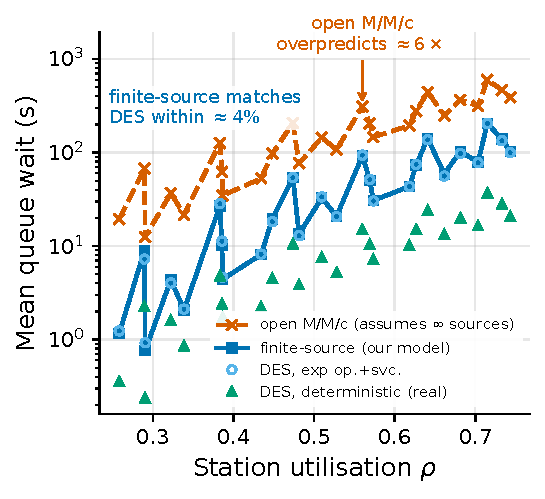
\includegraphics[width=\columnwidth]{../results/fig_des_validation.png}
%   \caption{Queue-model validation against discrete-event simulation.}
%   \label{fig:des}
% \end{figure}

%=======================================================================
\section{Conclusion}
\label{sec:concl}
% TODO.

\bibliographystyle{IEEEtran}
\bibliography{refs}   % <-- sub-agent fills refs.bib

\end{document}
